\documentclass[fleqn]{article}
\usepackage[utf8]{inputenc}
\usepackage[spanish, es-lcroman]{babel}
\usepackage[margin = 15mm]{geometry}
\usepackage{parskip}
\usepackage{amsmath, amssymb, amsfonts}
\usepackage{enumerate}
\usepackage{graphicx}

\expandafter\def\expandafter\normalsize\expandafter{%
    \setlength\abovedisplayskip{-9pt}%
    \setlength\belowdisplayskip{5pt}%
}

%\renewcommand{\theenumi}{\roman{enumi}}

\newcommand{\real}{\mathbb{R}}
\newcommand{\ent}{\mathbb{Z}}
\newcommand{\intg}[3]{\int_{#1}^{#2} #3 \, \mathrm{d}x}

\begin{document}
	\bfseries
	Ecuaciones Diferenciables Parciales \\
	Tarea 4 \\
	Osmar Dominique Santana Reyes \\
	No. de cuenta: 2125197 \\

	\begin{enumerate}[I.]
		\item Construya la serie de Fourier completa de la función dada $f$. En cada caso, utilice esquemas apropiados y analice la convergencia de la serie en el intervalo $ [-L,L] $ donde $f$ está definida.
		
		\begin{enumerate}[(1)]
			%----------------------------------------Ejercicio 1-------------------------------------------------------
			\item $ f(x) = \begin{cases}
				-2, & -1 \leq x \leq 0 \\
				3, & 0 < x \leq 1 \\
			\end{cases} $

			Solución.

			\normalfont

			\begin{equation*}
				a_0 = \dfrac{1}{1} \intg{-1}{1}{f(x)} = \intg{-1}{0}{-2} + \intg{0}{1}{3} = -2 + 3 = 1
			\end{equation*}

			\begin{equation*}
				a_n = \dfrac{1}{1} \intg{-1}{1}{f(x) \cos \left( \dfrac{n \pi x}{1} \right)} = \intg{-1}{0}{-2 \cos \left(n \pi x \right)} + \intg{0}{1}{3 \cos \left(n \pi x \right)} = 0
			\end{equation*}

			\begin{align*}
				b_n &= \dfrac{1}{1} \intg{-1}{1}{f(x) \sen \left( \dfrac{n \pi x}{1} \right)} = \intg{-1}{0}{-2 \sen \left(n \pi x \right)} + \intg{0}{1}{3 \sen \left(n \pi x \right)} \\
				&= \dfrac{2(1 - (-1)^n)}{n \pi} + \dfrac{3(-(-1)^n + 1)}{n \pi} = \dfrac{5(1 - (-1)^n)}{n \pi}
			\end{align*}

			Así, $ \displaystyle f(x) \sim \dfrac{1}{2} + \sum_{n=1}^{\infty} \dfrac{5(1 - (-1)^n)}{n \pi} \sen (n \pi x) $

			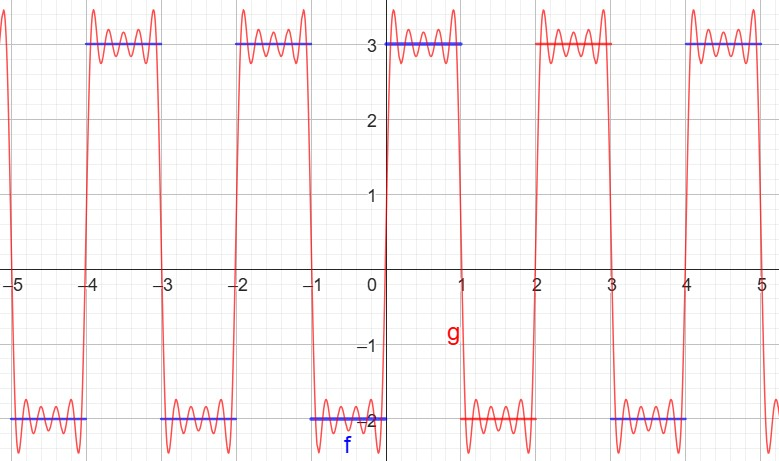
\includegraphics[width=0.95\linewidth]{Ejer1.jpg}

			Luego, como $f$ es suave por tramos en $ [-1,1] $, se tiene que la serie de fourier de $f$ converge puntualmente a la extensión periódica de $f$ a $ \real $ en todo $ x \in \real \setminus \ent $ y a $ \dfrac{f(x^-) + f(x^+)}{2} = \dfrac{3-2}{2} = \dfrac{1}{2} $ en todo $ x \in \ent $.

			%----------------------------------------Ejercicio 2-------------------------------------------------------

			\bfseries 
			\item $ f(x) = \begin{cases}
				x, & -1 \leq x \leq 0 \\
				2x - 1, & 0 < x \leq 1 \\
			\end{cases} $

			Solución.

			\normalfont

			\begin{equation*}
				a_0 = \dfrac{1}{1} \intg{-1}{1}{f(x)} = \intg{-1}{0}{x} + \intg{0}{1}{2x - 1} = -\dfrac{1}{2}
			\end{equation*}

			\begin{align*}
				a_n &= \dfrac{1}{1} \intg{-1}{1}{f(x) \cos \left( \dfrac{n \pi x}{1} \right)} = \intg{-1}{0}{x \cos \left(n \pi x \right)} + \intg{0}{1}{(2x - 1) \cos \left(n \pi x \right)} \\
				&= \dfrac{1 - (-1)^n}{\pi^2 n^2} + \dfrac{2((-1)^n - 1)}{\pi^2 n^2} = \dfrac{(-1)^n - 1}{\pi^2 n^2} 
			\end{align*}

			\begin{align*}
				b_n &= \dfrac{1}{1} \intg{-1}{1}{f(x) \sen \left( \dfrac{n \pi x}{1} \right)} = \intg{-1}{0}{x \sen \left(n \pi x \right)} + \intg{0}{1}{(2x - 1) \sen \left(n \pi x \right)} \\
				&= -\dfrac{(-1)^n}{n \pi} - \dfrac{(-1)^n + 1}{n \pi} = - \dfrac{2(-1)^n + 1}{n \pi}
			\end{align*}

			Así, $ \displaystyle f(x) \sim -\dfrac{1}{4} + \sum_{n=1}^{\infty} \left[ \dfrac{(-1)^n - 1}{\pi^2 n^2} \cos (n \pi x) - \dfrac{2(-1)^n + 1}{n \pi} \sen (n \pi x) \right] $

			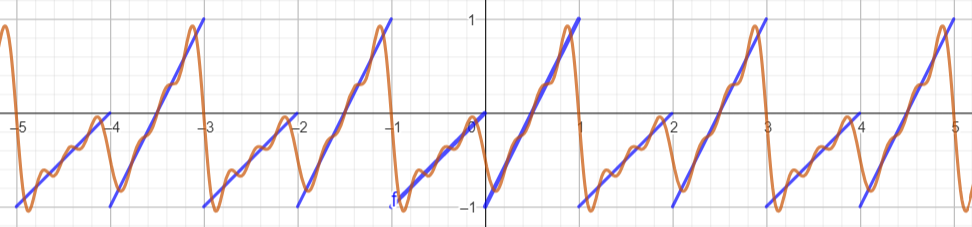
\includegraphics[width=0.95\linewidth]{Ejer2.png}

			Luego, como $f$ es suave por tramos en $ [-1,1] $, se tiene que la serie de fourier de $f$ converge puntualmente a la extensión periódica de $f$ a $ \real $ en todo $ x \in \real \setminus \ent $, a $ \dfrac{f(x^-) + f(x^+)}{2} = \dfrac{0-1}{2} = -\dfrac{1}{2} $ en todo $ x $ entero par y en $ \dfrac{f(x^-) + f(x^+)}{2} = \dfrac{1-1}{2} = 0 $ en todo $ x $ entero impar.

			%----------------------------------------Ejercicio 3-------------------------------------------------------

			\bfseries
			\item $ 1 - 2x, -2 \leq x \leq 2 $
			
			Solución.

			\normalfont

			\begin{equation*}
				a_0 = \dfrac{1}{2} \intg{-2}{2}{1 - 2x} = \dfrac{1}{2} (-2 + 6) = 2
			\end{equation*}

			\begin{equation*}
				a_n = \dfrac{1}{2} \intg{-2}{2}{(1 - 2x) \cos \left( \dfrac{n \pi x}{2} \right)} = 0
			\end{equation*}

			\begin{align*}
				b_n &= \dfrac{1}{2} \intg{-2}{2}{(1 - 2x) \sen \left( \dfrac{n \pi x}{2} \right)} = \dfrac{8(-1)^n}{n \pi}
			\end{align*}

			Así, $ \displaystyle f(x) \sim 1 + \sum_{n=1}^{\infty} \dfrac{8(-1)^n}{n \pi} \sen \left( \dfrac{n \pi x}{2} \right) $

			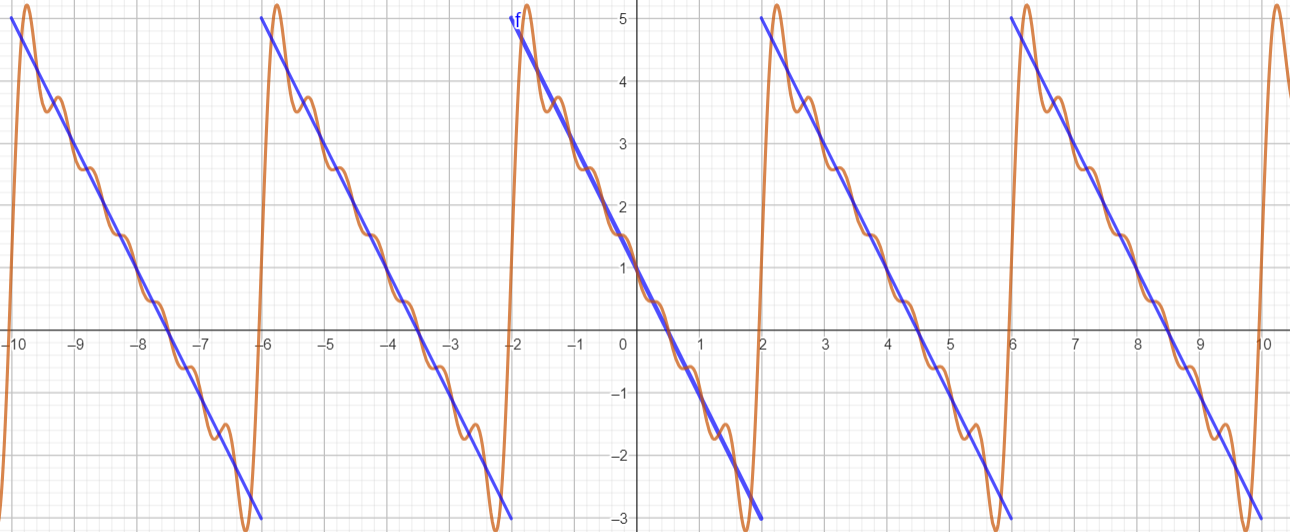
\includegraphics[width=0.95\linewidth]{Ejer3.png}

			Luego, como $f$ es suave por tramos en $ [-2,2] $, se tiene que la serie de fourier de $f$ converge puntualmente a la extensión periódica de $f$ a $ \real $ en todo $ x \in \real \setminus \{ x \in \ent \colon x \equiv 2 (\hspace{-2mm} \mod 4) \} $ y a $ \dfrac{f(x^-) + f(x^+)}{2} = \dfrac{-3+5}{2} = 1 $ en todo $ x \in \{ x \in \ent \colon x \equiv 2 (\hspace{-2mm} \mod 4) \} $.

			%----------------------------------------Ejercicio 4-------------------------------------------------------

			\bfseries
			\item $ f(x) = \begin{cases}
				x^2, & -1 \leq x \leq 0 \\
				1 + 2x, & 0 < x \leq 1 \\
			\end{cases} $

			Solución.

			\normalfont

			\begin{equation*}
				a_0 = \dfrac{1}{1} \intg{-1}{1}{f(x)} = \intg{-1}{0}{x^2} + \intg{0}{1}{1 + 2x} = \dfrac{1}{3} + 2 = \dfrac{7}{3}
			\end{equation*}

			\begin{align*}
				a_n &= \dfrac{1}{1} \intg{-1}{1}{f(x) \cos \left( \dfrac{n \pi x}{1} \right)} = \intg{-1}{0}{x^2 \cos \left(n \pi x \right)} + \intg{0}{1}{(1 + 2x) \cos \left(n \pi x \right)} \\
				&= \dfrac{2(-1)^n}{\pi^2 n^2} + \dfrac{2((-1)^n - 1)}{\pi^2 n^2} = \dfrac{4(-1)^n - 2}{\pi^2 n^2} 
			\end{align*}

			\begin{align*}
				b_n &= \dfrac{1}{1} \intg{-1}{1}{f(x) \sen \left( \dfrac{n \pi x}{1} \right)} = \intg{-1}{0}{x^2 \sen \left(n \pi x \right)} + \intg{0}{1}{(1 + 2x) \sen \left(n \pi x \right)} \\
				&= \dfrac{(-1)^n}{n \pi} + \dfrac{1 - 3(-1)^n}{n \pi} = \dfrac{1 - 2(-1)^n}{n \pi}
			\end{align*}

			Así, $ \displaystyle f(x) \sim \dfrac{7}{6} + \sum_{n=1}^{\infty} \left[ \dfrac{4(-1)^n - 2}{\pi^2 n^2} \cos (n \pi x) + \dfrac{1 - 2(-1)^n}{n \pi} \sen (n \pi x) \right] $

			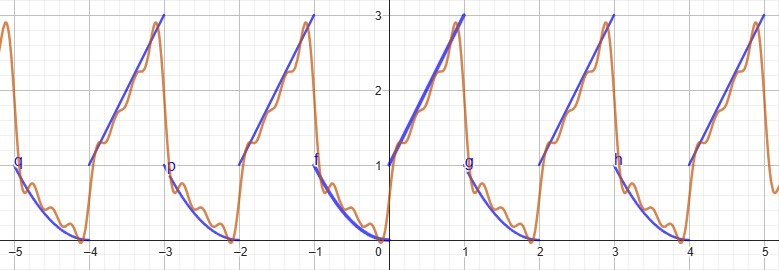
\includegraphics[width=0.95\linewidth]{Ejer4.jpg}

			Luego, como $f$ es suave por tramos en $ [-1,1] $, se tiene que la serie de fourier de $f$ converge puntualmente a la extensión periódica de $f$ a $ \real $ en todo $ x \in \real \setminus \ent $, a $ \dfrac{f(x^-) + f(x^+)}{2} = \dfrac{0+1}{2} = \dfrac{1}{2} $ en todo $ x $ entero par y en $ \dfrac{f(x^-) + f(x^+)}{2} = \dfrac{3+1}{2} = 2 $ en todo $ x $ entero impar.

			%----------------------------------------Ejercicio 5-------------------------------------------------------

			\bfseries
			\item $ f(x) = \begin{cases}
				0, & -2 \leq x \leq -1 \\
				1 + x, & -1 < x \leq 2 \\
			\end{cases} $
			
			Solución.

			\normalfont

			\begin{equation*}
				a_0 = \dfrac{1}{2} \intg{-2}{2}{f(x)} = \dfrac{1}{2} \intg{-2}{-1}{0} + \dfrac{1}{2} \intg{-1}{2}{1 + x} = \dfrac{9}{4}
			\end{equation*}

			\begin{align*}
				a_n &= \dfrac{1}{2} \intg{-2}{2}{f(x) \cos \left( \dfrac{n \pi x}{2} \right)} = \dfrac{1}{2} \intg{-2}{-1}{0 \cos \left( \dfrac{n \pi x}{2} \right)} + \dfrac{1}{2} \intg{-1}{2}{(1 + x) \cos \left( \dfrac{n \pi x}{2} \right)} \\
				&= \dfrac{-2}{\pi^2 n^2} \left( \cos \left( \dfrac{n \pi}{2} \right) - (-1)^n \right)
			\end{align*}

			\begin{align*}
				b_n &= \dfrac{1}{2} \intg{-2}{2}{f(x) \sen \left( \dfrac{n \pi x}{2} \right)} = \dfrac{1}{2} \intg{-2}{-1}{0 \sen \left( \dfrac{n \pi x}{2} \right)} + \dfrac{1}{2} \intg{-1}{2}{(1 + x) \sen \left( \dfrac{n \pi x}{2} \right)} \\
				&= \dfrac{-1}{n \pi} \left( 3(-1)^n + \dfrac{2}{n \pi} \sen \left( \dfrac{n \pi}{2} \right) \right)
			\end{align*}

			Así, $ \displaystyle f(x) \sim \dfrac{9}{8} - \sum_{n=1}^{\infty} \left[ \dfrac{2}{\pi^2 n^2} \left( \cos \left( \dfrac{n \pi}{2} \right) - (-1)^n \right) \cos \left( \dfrac{n \pi x}{2} \right) + \dfrac{1}{n \pi} \left( 3(-1)^n + \dfrac{2}{n \pi} \sen \left( \dfrac{n \pi}{2} \right) \right) \sen \left( \dfrac{n \pi x}{2} \right) \right] $

			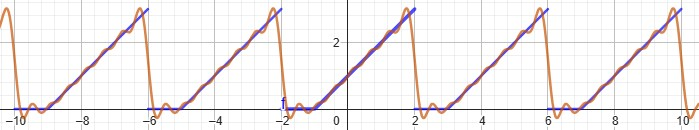
\includegraphics[width=0.95\linewidth]{Ejer5.jpg}

			Luego, como $f$ es suave por tramos en $ [-2,2] $, se tiene que la serie de fourier de $f$ converge puntualmente a la extensión periódica de $f$ a $ \real $ en todo $ x \in \real \setminus \{ x \in \ent \colon x \equiv 2 (\hspace{-2mm} \mod 4) \} $ y en $ \dfrac{f(x^-) + f(x^+)}{2} = \dfrac{3+0}{2} = \dfrac{3}{2} $ en todo $ x \in \{ x \in \ent \colon x \equiv 2 (\hspace{-2mm} \mod 4) \} $.

			\bfseries
		\end{enumerate}

		\item Construya la serie de senos de Fourier y la serie de cosenos de Fourier de la función dada $f$. En cada caso, utilice esquemas apropiados y analice la convergencia de la serie en el intervalo $ [0,L] $ donde $f$ está definida.
		
		\begin{enumerate}[(1)]
			%----------------------------------------Ejercicio 6-------------------------------------------------------
			\item $ f(x) = \begin{cases}
				0, & 0 \leq x \leq 1 \\
				1, & 1 < x \leq 2 \\
			\end{cases} $

			Solución.

			\normalfont

			\begin{equation*}
				a_0 = \dfrac{1}{2} \intg{0}{2}{f(x)} = \dfrac{1}{2} \intg{0}{1}{0} + \dfrac{1}{2} \intg{1}{2}{1} = \dfrac{1}{2}
			\end{equation*}

			\begin{equation*}
				a_n = \dfrac{2}{2} \intg{0}{2}{f(x) \cos \left( \dfrac{n \pi x}{2} \right)} = \intg{0}{1}{0 \cos \left( \dfrac{n \pi x}{2} \right)} + \intg{1}{2}{\cos \left( \dfrac{n \pi x}{2} \right)} = \dfrac{-2}{n \pi} \sen \left( \dfrac{n \pi}{2} \right)
			\end{equation*}

			\begin{align*}
				b_n &= \dfrac{2}{2} \intg{-1}{1}{f(x) \sen \left( \dfrac{n \pi x}{2} \right)} = \intg{0}{1}{0 \sen \left( \dfrac{n \pi x}{2} \right)} + \intg{1}{2}{\sen \left( \dfrac{n \pi x}{2} \right)} \\
				&= \dfrac{2}{n \pi} \left( \cos \left( \dfrac{n \pi}{2} \right) - (-1)^n \right)
			\end{align*}

			Así, la serie de senos de $ f $ es: $ \displaystyle \sum_{n=1}^{\infty} \dfrac{2}{n \pi} \left( \cos \left( \dfrac{n \pi}{2} \right) - (-1)^n \right) \sen \left( \dfrac{n \pi x}{2} \right) $.

			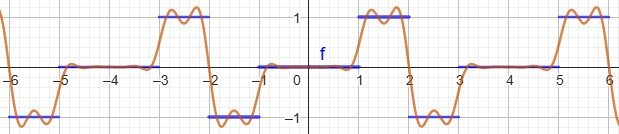
\includegraphics[width=0.95\linewidth]{Ejer6s.jpg}

			Después, ya que $f$ es suave por tramos en $ [-2,2] $, se tiene que la serie de senos de fourier de $f$ converge puntualmente a la extensión periódica de $f$ a $ \real $ en todo $ x \in \real \setminus \{ x \in \ent \colon x \neq 4n, \mbox{ con } n \in \ent \} $ y en

			\begin{itemize}
				\item $ \dfrac{f(x^-) + f(x^+)}{2} = \dfrac{0+1}{2} = \dfrac{1}{2} $ para todo $ x \in \{ x \in \ent \colon x \equiv 1 (\hspace{-2mm} \mod 4) \} $.
				
				\item $ \dfrac{f(x^-) + f(x^+)}{2} = \dfrac{1-1}{2} = 0 $ para todo $ x \in \{ x \in \ent \colon x \equiv 2 (\hspace{-2mm} \mod 4) \} $.
				
				\item $ \dfrac{f(x^-) + f(x^+)}{2} = \dfrac{-1+0}{2} = -\dfrac{1}{2} $ para todo $ x \in \{ x \in \ent \colon x \equiv 3 (\hspace{-2mm} \mod 4) \} $.
			\end{itemize}

			Por otro lado, la serie de cosenos es: $ \displaystyle \dfrac{1}{2} - \sum_{n=1}^{\infty} \dfrac{2}{n \pi} \sen \left( \dfrac{n \pi}{2} \right) \cos \left( \dfrac{n \pi x}{2} \right) $.

			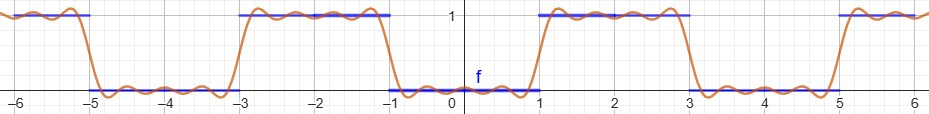
\includegraphics[width=0.95\linewidth]{Ejer6c.jpg}

			Luego, ya que $f$ es suave por tramos en $ [-2,2] $, se tiene que la serie de cosenos de fourier de $f$ converge puntualmente a la extensión periódica de $f$ a $ \real $ en todo $ x \in \real \setminus \{ x \in \ent \colon x = 2n-1, \mbox{ con } n \in \ent \} $ y en $ \dfrac{f(x^-) + f(x^+)}{2} = \dfrac{0+1}{2} = \dfrac{1}{2} $ para todo $ x \in \{ x \in \ent \colon x = 2n-1, \mbox{ con } n \in \ent \} $.

			%----------------------------------------Ejercicio 7-------------------------------------------------------

			\bfseries
			\item $ f(x) = \begin{cases}
				-2, & 0 \leq x \leq \dfrac{\pi}{2} \\
				3, & \dfrac{\pi}{2} < x \leq \pi \\
			\end{cases} $

			Solución.

			\normalfont

			\begin{equation*}
				a_0 = \dfrac{1}{\pi} \intg{0}{\pi}{f(x)} = \dfrac{1}{\pi} \intg{0}{\frac{\pi}{2}}{-2} + \dfrac{1}{\pi} \intg{\frac{\pi}{2}}{\pi}{3} = -1 + \dfrac{3}{2} = \dfrac{1}{2}
			\end{equation*}

			\begin{align*}
				a_n &= \dfrac{2}{\pi} \intg{0}{\pi}{f(x) \cos \left( \dfrac{n \pi x}{\pi} \right)} = \dfrac{2}{\pi} \intg{0}{\frac{\pi}{2}}{-2 \cos \left( n x \right)} + \dfrac{2}{\pi} \intg{\frac{\pi}{2}}{\pi}{3 \cos \left( n x \right)} \\
				&= -\dfrac{4}{n \pi} \sen \left( \dfrac{n \pi}{2} \right) - \dfrac{6}{n \pi} \sen \left( \dfrac{n \pi}{2} \right) = - \dfrac{10}{n \pi} \sen \left( \dfrac{n \pi}{2} \right)
			\end{align*}

			\begin{align*}
				b_n &= \dfrac{2}{\pi} \intg{0}{\pi}{f(x) \sen \left( \dfrac{n \pi x}{\pi} \right)} = \dfrac{2}{\pi} \intg{0}{\frac{\pi}{2}}{-2 \sen \left( n x \right)} + \dfrac{2}{\pi} \intg{\frac{\pi}{2}}{\pi}{3 \sen \left( n x \right)} \\
				&= \dfrac{4}{n \pi} \left( \cos \left( \dfrac{n \pi}{2} \right) - 1 \right) + \dfrac{6}{n \pi} \left( \cos \left( \dfrac{n \pi}{2} \right) - (-1)^n \right) = \dfrac{2}{n \pi} \left( 5 \cos \left( \dfrac{n \pi}{2} \right) - 3(-1)^n - 2 \right)
			\end{align*}

			Así, la serie de senos de $ f $ es: $ \displaystyle \sum_{n=1}^{\infty} \dfrac{2}{n \pi} \left( 5 \cos \left( \dfrac{n \pi}{2} \right) - 3(-1)^n - 2 \right) \sen (n x) $.

			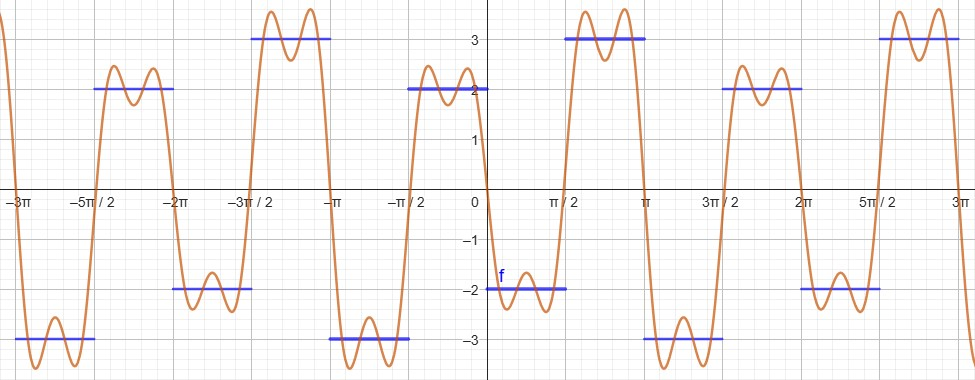
\includegraphics[width=0.95\linewidth]{Ejer7s.jpg}

			Después, ya que $f$ es suave por tramos en $ [-\pi,\pi] $, se tiene que la serie de senos de fourier de $f$ converge puntualmente a la extensión periódica de $f$ a $ \real $ en todo $ x \in \real \setminus \left\lbrace x \in \real \colon x = \dfrac{n \pi}{2}, \mbox{ con } n \in \ent \right\rbrace $ y en

			\begin{itemize}
				\item $ \dfrac{f(x^-) + f(x^+)}{2} = \dfrac{2-2}{2} = 0 $ para todo $ x \in \{ x \in \real \colon x = 2n \pi, \mbox{ con } n \in \ent \} $.
				
				\item $ \dfrac{f(x^-) + f(x^+)}{2} = \dfrac{-2+3}{2} = \dfrac{1}{2} $ para todo $ x \in \left\lbrace x \in \real \colon x = (4n + 1) \dfrac{\pi}{2}, \mbox{ con } n \in \ent \right\rbrace $.
				
				\item $ \dfrac{f(x^-) + f(x^+)}{2} = \dfrac{3-3}{2} = 0 $ para todo $ x \in \left\lbrace x \in \real \colon x = (2n + 1) \pi, \mbox{ con } n \in \ent \right\rbrace $.
				
				\item $ \dfrac{f(x^-) + f(x^+)}{2} = \dfrac{-3+2}{2} = -\dfrac{1}{2} $ para todo $ x \in \left\lbrace x \in \real \colon x = (4n + 3) \dfrac{\pi}{2}, \mbox{ con } n \in \ent \right\rbrace $.
			\end{itemize}

			Por otro lado, la serie de cosenos es: $ \displaystyle \dfrac{1}{2} - \sum_{n=1}^{\infty} \dfrac{10}{n \pi} \sen \left( \dfrac{n \pi}{2} \right) \cos (n x) $.

			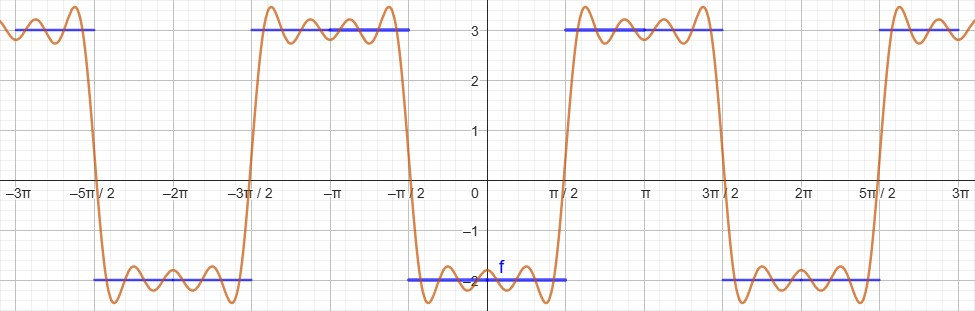
\includegraphics[width=0.95\linewidth]{Ejer7c.jpg}

			Luego, ya que $f$ es suave por tramos en $ [-\pi,\pi] $, se tiene que la serie de cosenos de fourier de $f$ converge puntualmente a la extensión periódica de $f$ a $ \real $ en todo $ x \in \real \setminus \left\lbrace x \in \real \colon x = (2n+1) \dfrac{\pi}{2}, \mbox{ con } n \in \ent \right\rbrace $ y en $ \dfrac{f(x^-) + f(x^+)}{2} = \dfrac{-2+3}{2} = \dfrac{1}{2} $ para todo $ x \in \left\lbrace x \in \real \colon x = (2n+1) \dfrac{\pi}{2}, \mbox{ con } n \in \ent \right\rbrace $.

			%----------------------------------------Ejercicio 8-------------------------------------------------------

			\bfseries
			\item $ f(x) = \begin{cases}
				x, & 0 \leq x \leq 1 \\
				-2, & 1 < x \leq 2 \\
			\end{cases} $

			Solución.

			\normalfont

			\begin{equation*}
				a_0 = \dfrac{1}{2} \intg{0}{2}{f(x)} = \dfrac{1}{2} \intg{0}{1}{x} + \dfrac{1}{2} \intg{1}{2}{-2} = \dfrac{1}{4} - 1 = -\dfrac{3}{4}
			\end{equation*}

			\begin{align*}
				a_n &= \dfrac{2}{2} \intg{0}{2}{f(x) \cos \left( \dfrac{n \pi x}{2} \right)} = \intg{0}{1}{x \cos \left( \dfrac{n \pi x}{2} \right)} + \intg{1}{2}{-2 \cos \left( \dfrac{n \pi x}{2} \right)} \\
				&= \dfrac{2}{n^2 \pi^2} \left( n \pi \sen \left( \dfrac{n \pi}{2} \right) + 2 \cos \left( \dfrac{n \pi}{2} \right) - 2 \right) + \dfrac{4}{n \pi} \sen \left( \dfrac{n \pi}{2} \right) = \dfrac{2}{n^2 \pi^2} \left( 3n \pi \sen \left( \dfrac{n \pi}{2} \right) + 2 \cos \left( \dfrac{n \pi}{2} \right) - 2 \right)
			\end{align*}

			\begin{align*}
				b_n &= \dfrac{2}{2} \intg{0}{2}{f(x) \sen \left( \dfrac{n \pi x}{2} \right)} = \intg{0}{1}{x \sen \left( \dfrac{n \pi x}{2} \right)} + \intg{1}{2}{-2 \sen \left( \dfrac{n \pi x}{2} \right)} \\
				&= \dfrac{2}{n^2 \pi^2} \left( 2 \sen \left( \dfrac{n \pi}{2} \right) - n \pi \cos \left( \dfrac{n \pi}{2} \right) \right) + \dfrac{4}{n \pi} \left( (-1)^n - \cos \left( \dfrac{n \pi}{2} \right) \right) \\
				&= \dfrac{2}{n^2 \pi^2} \left( 2 \sen \left( \dfrac{n \pi}{2} \right) - 3n \pi \cos \left( \dfrac{n \pi}{2} \right) + 2 \pi n (-1)^n \right)
			\end{align*}

			Así, la serie de senos de $ f $ es: $ \displaystyle \sum_{n=1}^{\infty} \dfrac{2}{n^2 \pi^2} \left( 2 \sen \left( \dfrac{n \pi}{2} \right) - 3n \pi \cos \left( \dfrac{n \pi}{2} \right) + 2 \pi n (-1)^n \right) \sen \left( \dfrac{n \pi x}{2} \right) $.

			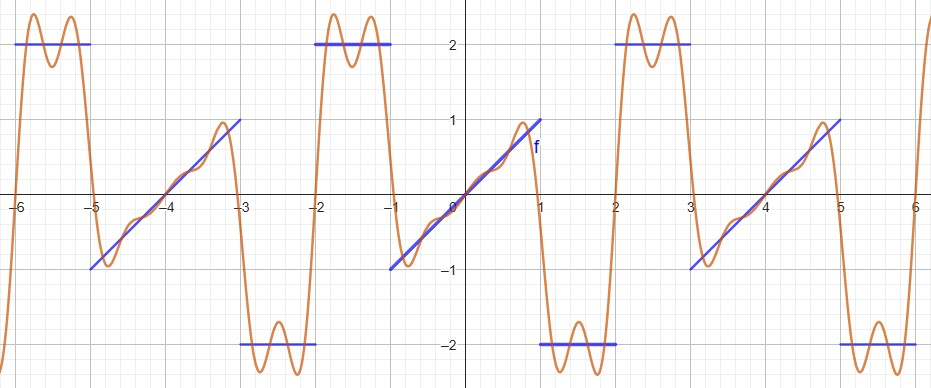
\includegraphics[width=0.95\linewidth]{Ejer8s.jpg}

			Después, ya que $f$ es suave por tramos en $ [-\pi,\pi] $, se tiene que la serie de senos de fourier de $f$ converge puntualmente a la extensión periódica de $f$ a $ \real $ en todo $ x \in \real \setminus \left\lbrace x \in \real \colon x = \dfrac{n \pi}{2}, \mbox{ con } n \in \ent \right\rbrace $ y en

			\begin{itemize}
				\item $ \dfrac{f(x^-) + f(x^+)}{2} = \dfrac{2-2}{2} = 0 $ para todo $ x \in \{ x \in \real \colon x = 2n \pi, \mbox{ con } n \in \ent \} $.
				
				\item $ \dfrac{f(x^-) + f(x^+)}{2} = \dfrac{-2+3}{2} = \dfrac{1}{2} $ para todo $ x \in \left\lbrace x \in \real \colon x = (4n + 1) \dfrac{\pi}{2}, \mbox{ con } n \in \ent \right\rbrace $.
				
				\item $ \dfrac{f(x^-) + f(x^+)}{2} = \dfrac{3-3}{2} = 0 $ para todo $ x \in \left\lbrace x \in \real \colon x = (2n + 1) \pi, \mbox{ con } n \in \ent \right\rbrace $.
				
				\item $ \dfrac{f(x^-) + f(x^+)}{2} = \dfrac{-3+2}{2} = -\dfrac{1}{2} $ para todo $ x \in \left\lbrace x \in \real \colon x = (4n + 3) \dfrac{\pi}{2}, \mbox{ con } n \in \ent \right\rbrace $.
			\end{itemize}

			Por otro lado, la serie de cosenos es: $ \displaystyle \dfrac{1}{2} - \sum_{n=1}^{\infty} \dfrac{10}{n \pi} \sen \left( \dfrac{n \pi}{2} \right) \cos (n x) $.

			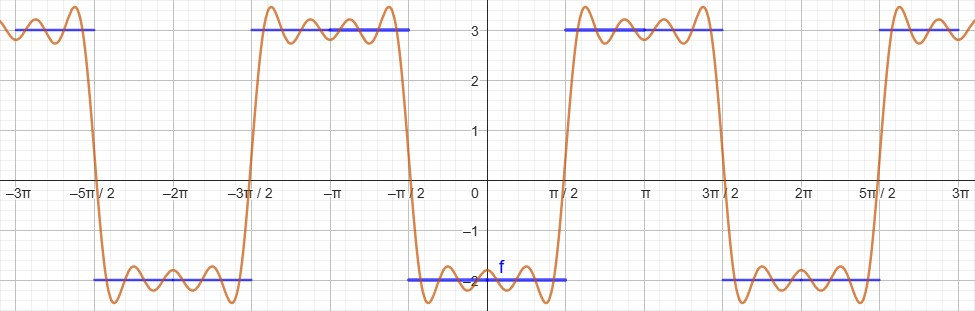
\includegraphics[width=0.95\linewidth]{Ejer7c.jpg}

			Luego, ya que $f$ es suave por tramos en $ [-\pi,\pi] $, se tiene que la serie de cosenos de fourier de $f$ converge puntualmente a la extensión periódica de $f$ a $ \real $ en todo $ x \in \real \setminus \left\lbrace x \in \real \colon x = (2n+1) \dfrac{\pi}{2}, \mbox{ con } n \in \ent \right\rbrace $ y en $ \dfrac{f(x^-) + f(x^+)}{2} = \dfrac{-2+3}{2} = \dfrac{1}{2} $ para todo $ x \in \left\lbrace x \in \real \colon x = (2n+1) \dfrac{\pi}{2}, \mbox{ con } n \in \ent \right\rbrace $.

			%----------------------------------------Ejercicio 9-------------------------------------------------------

			\bfseries
			\item $ f(x) = \begin{cases}
				\cos (x), & 0 \leq x \leq \dfrac{\pi}{2} \\
				-1, & \dfrac{\pi}{2} < x \leq \pi \\
			\end{cases} $

			Solución.

			\normalfont



			%----------------------------------------Ejercicio 10-------------------------------------------------------

			\bfseries
			\item $ f(x) = x + \sen (x), 0 \leq x \leq \pi $
			
			Solución.

			\normalfont



		\end{enumerate}
	\end{enumerate}
\end{document}